
\section{Theorie}
\label{sec:Theorie}
\subsection{Der Brechungsindex}
Es ist bekannt, dass die Lichtgeschwindigkeit eine feste Größe ist und ca. $\SI{3 E8}{\meter\per\second}$ beträgt. Hierbei handelt es sich jedoch um die die Lichtgeschwindigkeit im Vakuum. In Materie hat Licht hingegen eine materialspezifische Geschwindigkeit, welche kleiner ausfällt. Anders betrachtet verlängert sich der optische Weg in einem Medium. Der Brechungsindex gibt das Verhältnis der Lichtgeschwindigkeit in Materie zur Lichtgeschwindigkeit im Vakuum an. Daher gilt:
\begin{equation}
    n = \frac{c_\text{Materie}}{c_\text{Vakuum}} \label{eq:n} \text{.}
\end{equation}  

 \subsection{Die Bestimmung des Brechungsindex von Gasen}
 Eine Methode den Brechungsindex bei Gasen zu bestimmen, ist die Dichte des untersuchten Gases zunächst zu reduzieren und den Druck nachher wieder langsam zu erhöhen. Wird das Gas dabei in den Lichtweg eines Interferometers gebracht, sorgt die dynamisch ansteigende optische Weglänge dazu, dass beide Strahlen am Ende miteinander interferieren und es zu Intensitätsmaxima und Minima kommt. Dies wird bei Verwendung des Wellenmodells des Lichtes deutlich. 
 In der klassischen Darstellung wird Licht als Überlagerung ebener Wellen dargestellt. Wird zusätzlich linear polarisiertes Licht angenommen, kann Die Welle durch
 \begin{equation}
    f(x,t) = exp(i \frac{2 \pi}{\lambda_\text{Vakuum}} n x ) e^{(-i \omega t)} \label{eq:ebeneWelle}
 \end{equation}
dargestellt werden. Kommt es nun zu einer Änderung des Brechungsindex über eine Länge $L$,so führt dies zu einer Phasenverschiebung der Welle. Bei einem Vakuumbrechungsindex von eins folgt:
\begin{equation}
    \Delta \varphi = \frac{2 \pi}{\lambda_\text{Vakuum}} (n-1) L \text{.} \label{eq:Deltaphi}
\end{equation}
Der Brechungsindex eines Gases beziehungsweise einer Flüssigkeit in Abhängigkeit des Druckes, der Temperatur und der Polarisierbarkeit lässt sich gut durch das Lorenz-Lorentz Gesetz beschreiben. Es ist zudem möglich die Eigenschaften von Gas oder Flüssigkeitsgemischen zu bestimmen, indem die Eigenschaften der einzelnen Komponenten bestimmt werden.

\begin{figure}
	\centering
	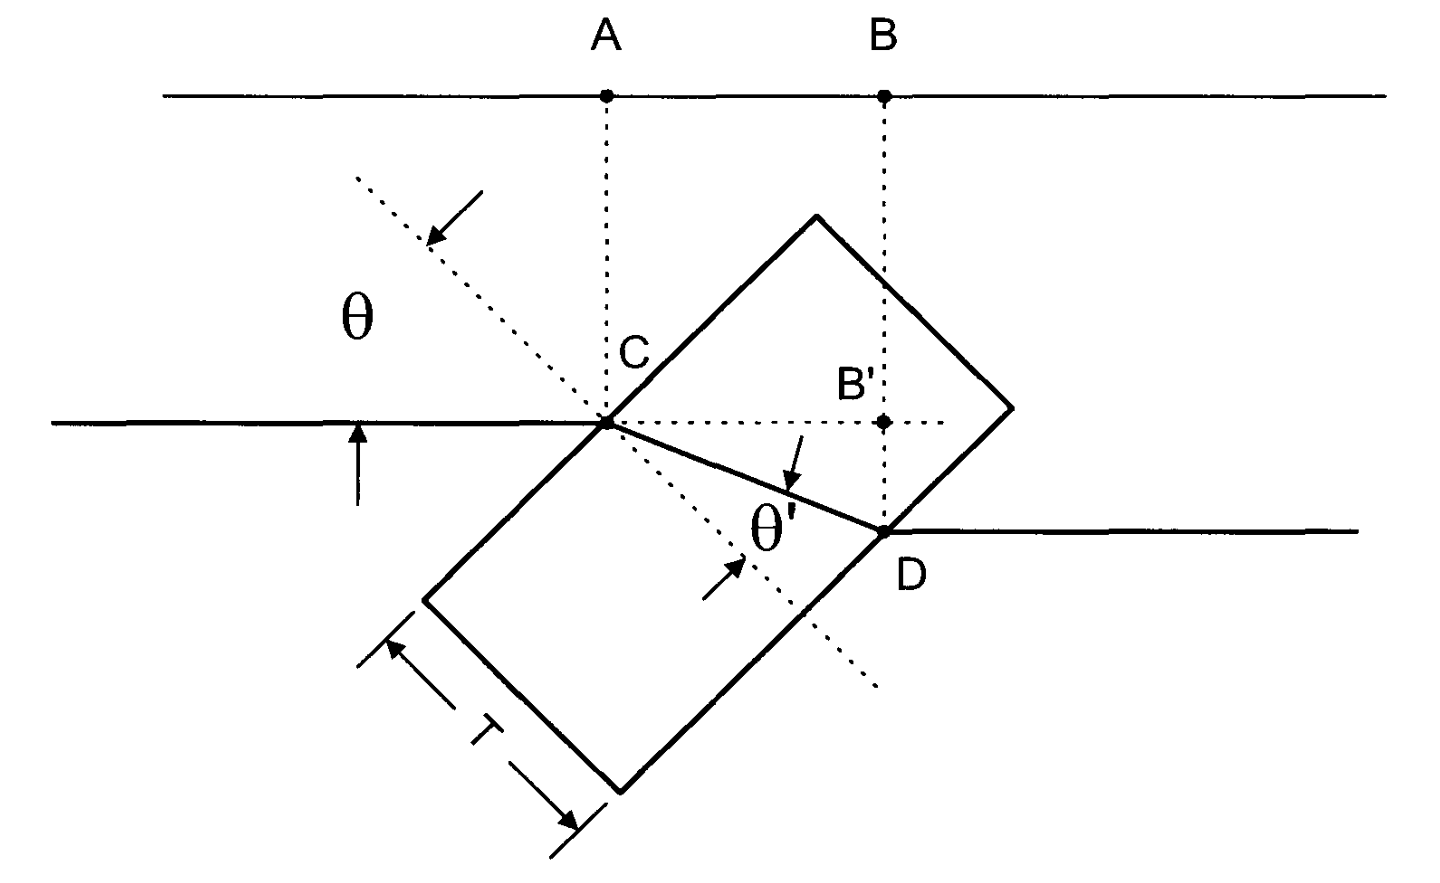
\includegraphics[width=\linewidth-100pt,height=\textheight-100pt,keepaspectratio]{content/Bilder/drehscheibeskizze.png}
	\caption{Hilfsskizze zur Bestimmung des optischen Weges einer rotierender Scheibe \cite{V64}.}
	\label{fig:Drehscheibe}
\end{figure}

\subsection{Die Bestimmung des Brechungsindex von lichtdurchlässigen Festkörpern}
Im Falle eines Festkörpers kann die Dichte nicht einfach variiert werden. Daher wird eine dünne Scheibe der Dicke $T$ des Materials auf eine drehbare Bühne gesetzt. Wird die Probe nun gedreht, verlängert sich der optische Lichtweg gemäß Abb. \ref{fig:Drehscheibe} wieder kontinuierlich. Wird die drehbare Bühne nun in das Interferometer gesetzt folgt für den auftretenden Phasenunterschied:
\begin{equation}
    \varphi(\theta) = \frac{2 \pi}{c_\text{Vakuum}} T \left( \frac{n - \cos(\theta - \theta ')}{\cos(\theta')} - n + 1 \right) \text{.} \label{eq:phi}
\end{equation}

Für den Brechungsindex folgt:
\begin{equation}
 n_\text{Glas} = \frac{\alpha^2 + 2 (\cos(\theta_1)-\cos(\theta_2))(1-\alpha)}{2 (\cos(\theta_1)-\cos(\theta_2)-\alpha)} \label{eq:glas}
\end{equation}
mit $\alpha = M \lambda_\text{vac}/(2 T)$.


\begin{figure}
	\centering
	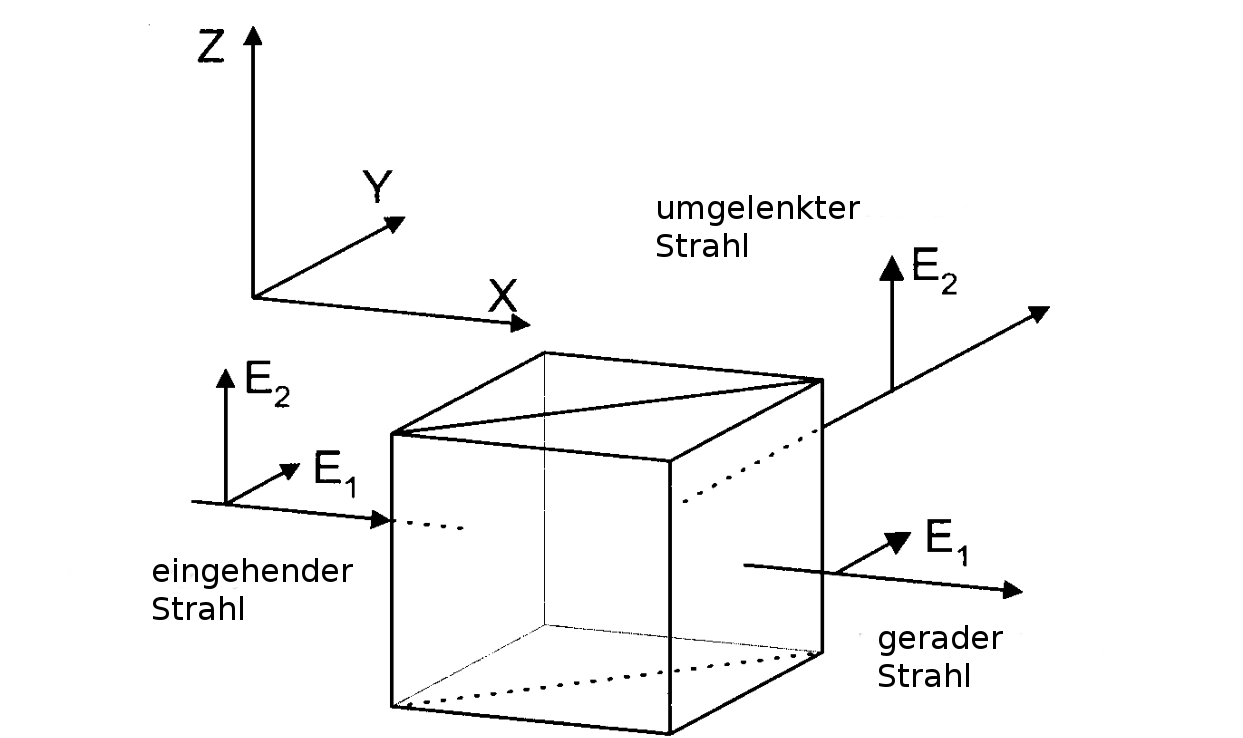
\includegraphics[width=\linewidth-100pt,height=\textheight-100pt,keepaspectratio]{content/Bilder/PBSC.png}
	\caption{Skizzierung der Wirkungsweise eines PBSC \cite{V64}.}
	\label{fig:PBSC}
\end{figure}


\subsection{Die Polarisation von Licht}
Licht besteht aus einer Überlagerung vieler verschiedener einzelner Wellen. Wird nun ein Polarisationsfilter in den Strahlengang gebracht, filtert dieser alle Komponenten des Lichtes heraus, welche orthogonal zum Polarisationsrichtung des Filters verlaufen. Daher verbleibt nur ein linear polarisierter Strahl übrig. Die Wirkung des PBSC ist eine ähnliche. Dieser gemäß Abb. \ref{fig:PBSC} aus zwei Glasprismen und lässt eine Polarisationsrichtung des Strahles passieren, während die dazu orthogonale um $\SI{90}{\degree}$ abgelenkt wird.

\subsection{Definition des Kontrastes}
Der Kontrast gibt ein Verhältnis zwischen maximaler $I_\text{max}$ und minimaler Intensität $I_\text{min}$an. Er ist definiert durch:
\begin{equation}
    K = \frac{I_\text{max} - I_\text{min}}{I_\text{max} + I_\text{min}} \text{.}          \label{eq:kont}
\end{equation}